\documentclass[dvipsnames,tikz]{standalone}
\usepackage{amsmath}
\usepackage{xcolor}
\usepackage{tikz}
\usetikzlibrary{calc}
\usetikzlibrary{decorations.pathreplacing,calligraphy,3d}


\begin{document}
	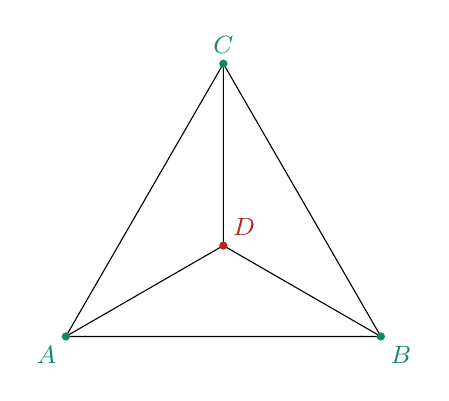
\begin{tikzpicture}[font=\small]
		\draw (0,0) -- (4,0) -- (2,3.464) -- cycle;
		\draw (0,0)-- (2,1.154) -- (2,3.464);
		\draw (2,1.154)-- (4,0);
		
		\fill[PineGreen] (0,0) circle (1.5pt) node [below left] {$A$};
		\fill[PineGreen] (4,0) circle (1.5pt) node [below right] {$B$};
		\fill[PineGreen] (2,3.464) circle (1.5pt) node [above] {$C$};
		\fill[BrickRed] (2,1.154) circle (1.5pt) node [above right] {$D$};
	\end{tikzpicture}
\end{document}